\documentclass[pdftex]{article}
\usepackage{times}
\usepackage{amsmath}
\usepackage{amsfonts}
\usepackage{fancyhdr}
\usepackage{amssymb}
\usepackage{verbatim}
\usepackage{graphicx}
\usepackage{float}
\usepackage{multicol}
\usepackage[section]{placeins}
\usepackage[margin=1.0in]{geometry}
\usepackage[numbered=true]{bookmark}

\begin{document}

\fancyhead[L]{PRELIMINARY}
\fancyfoot[L]{Revision: 0.1/PRELIMINARY}
\pagestyle{fancy}

\title{RED TIN Internal Logic Analyzer Datasheet\\Revision 0.1}
\author{Andrew D. Zonenberg\\
	\texttt{azonenberg@drawersteak.com}}
\date{\today}
\maketitle

\paragraph*{}
{\bf NOTE: } This document is preliminary and is subject to change. The software/firmware described in this document is
an alpha release which may contain bugs or errata. While a best effort attempt has been made to list all known errata
in this document, comprehensive testing has not yet been completed.

\paragraph*{}
Bug reports are welcomed. Please email reports to the email address listed on this title page.

\pagebreak
\tableofcontents
\pagebreak

\pagebreak
\section{Introduction} 

\paragraph*{}
RED TIN is an internal logic analyzer for debugging FPGA designs. It consists of three components - the capture module,
the interface wrapper, and the user interface. The first two are Verilog modules that run on the DUT FPGA and the last
is a C++ GUI application.

\paragraph*{}
RedTinLogicAnalyzer, the {\bf capture module}, is responsible for sampling data from the DUT and storing it to a
N-sample circular buffer. When waiting for a trigger event the buffer is continually rotating and data is written to the
Mth position in the buffer. Once triggered the start and stop pointers are frozen and data is stored until the end of
the buffer is reached. This results in M samples before the trigger and (N-M) after. Currently N and M have values of
512 and 16, respectively. In a future release the depth N will likely be parameterizable, and the the value of M will be
adjustable at run time between captures. The sample width is currently hardcoded to 128 (partial parameterization
has been implemented; the beta release will either complete or remove this).

\paragraph*{}
The {\bf interface wrapper} is responsible for bridging communications from the capture module to a PC. The interface
may be anything supported by the target board; currently only a UART at 500kbaud is implemented (RedTinUARTWrapper).
Future releases may add support for other interfaces such as JTAG, Ethernet, USB.

\paragraph*{}
The {\bf user interface} allows the user to specify the signals and trigger parameters to be used by the system. Once
a capture has completed, the UI reformats the raw binary data dump into a standard .vcd file and displays it in a
third-party waveform viewer. This is currently gtkwave (hard coded) however support for additional viewers will be
added in a future release.

\paragraph*{}
The Verilog components have only been tested on a Xilinx Spartan-6 FPGA, but were written in a portable fashion and
should be usable with any Verilog toolchain. Reports of successful or failed tests on other platforms are welcome.

\paragraph*{}
The UI application was written in C++ using the gtkmm GUI framework and should be easy to port to other platforms
however the alpha release has only been tested on 64-bit Debian ``Squeeze". The UART communications code is currently
not as modular as desirable; a future refactoring will make it easier to add suport for new bridges or interface APIs.
Reports of successful or failed tests on other platforms are welcome.

\paragraph*{}
The name ``RED TIN" has no meaning whatsoever. It was chosen by the following algorithm (used when nobody involved can
think of something that sounds good):
\begin{verbatim}
do
{
  a = random adjective
  n = random noun
} while(!sounds_good(a + " " + n))
\end{verbatim}

\pagebreak
\section{Capture module usage}

\paragraph*{}
Integration of the capture module into an existing FPGA design is quite simple. Simply create an instance of the
appropriate capture wrapper (RedTinUARTWrapper is the only one implemented in the alpha), connect the ``clk" input
to the sampling clock, and connect the signals of interest to the ``din" input. Any additional signals are dependent on
the specific wrapper interface and should be connected as mentioned in the documentation for that wrapper.

\section{User interface operation}

\paragraph*{}
The user interface consists of two panels separated by a splitter bar. The left panel is used to define the signals
being observed and the right panel is used to specify triggers and capture parameters.

\paragraph*{}
\begin{figure}[h]
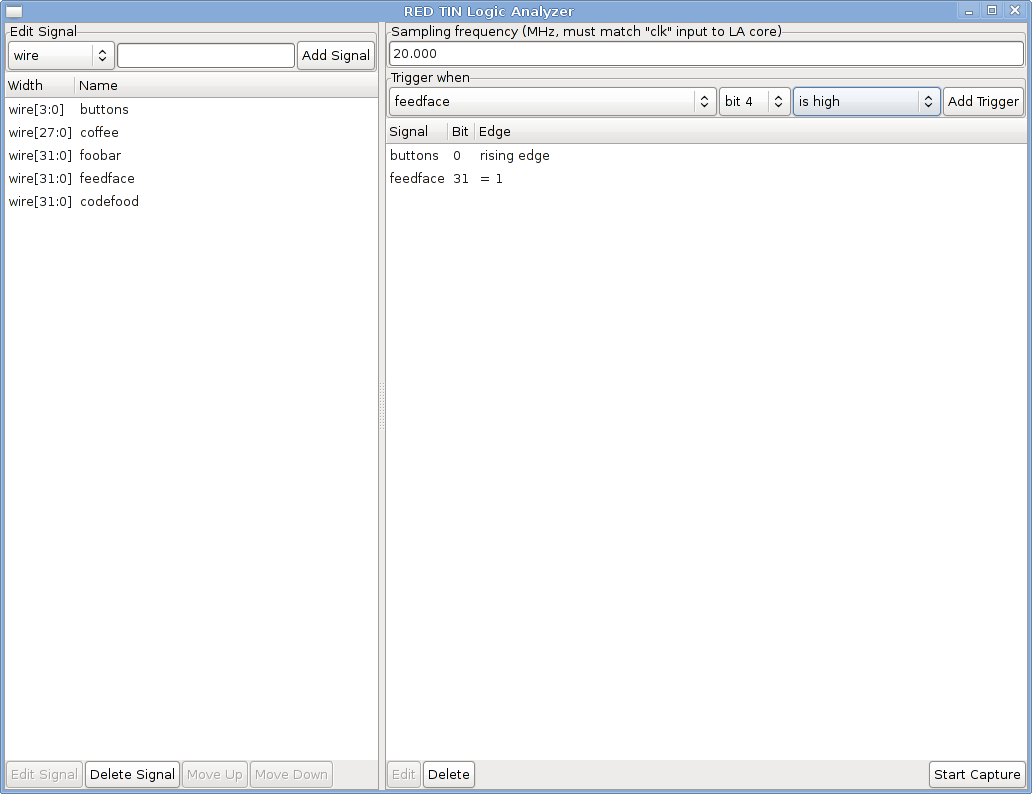
\includegraphics[scale=0.45]{gui-shot1.png}
\caption{Screenshot of UI}
\label{gui-overview}
\end{figure}

\subsection{Signals}
\paragraph*{}
To define the signals being watched, select the width from the drop-down box at the top of the left-hand panel,
give the signal a name, and click the ``add signal" button. The high-order bit of the first signal is mapped to
din[127] of the capture module and subsequent signals are packed in from left to right.

\paragraph*{}
In the alpha release, although signals can be deleted from the list, there is no support for editing or reordering
signals. Any error requires deleting and re-adding the affected signals.

\subsection{Triggers}
\paragraph*{}
To create a trigger, select the signal of interest from the ``trigger when" dropdown list, select the bit of interest,
specify the desired state (high, low, rising edge, falling edge, or change), and click the ``add trigger" button. Note
that ALL trigger conditions must hold simultaneously to trigger the logic analyzer. There is currently no support for
multiple sets of conditions however this may be added in a future release.

\subsection{Capturing}
\paragraph*{}
To begin a capture, verify the sampling frequency specified in the UI matches the ``clk" frequency supplied to the
capture module; then click the ``start capture" button. Once the trigger condition has occurred, the waveform viewer
will be launched to view the captured data.

\paragraph*{}
In the alpha, the source of capture data is hard coded to be a UART on /dev/ttyUSB0 and cannot be changed except by
recompiling the UI application.

\paragraph*{}
There is no support in the alpha release for canceling a pending capture. This will be added in a future release.

\subsection{Signal configuration files}
\paragraph*{}
When closing the UI, a prompt is displayed allowing the list of signals and triggers to be saved to a .scfg (signal
configuration) file. To load a saved scfg file, simply pass the filename as the first argument to the ``redtin" binary.

\pagebreak
\section{Writing a new wrapper module}

\paragraph*{}
This section will be written after a stable API for wrapper modules has been developed, most likely in time for an
Alpha 2 or Beta release.

\pagebreak
\section{Protocol descriptions}

\subsection{UART wrapper}

\paragraph*{}
This section will be written in a later release.

\pagebreak
\section{Errata}

\paragraph*{}
All known bugs were fixed before the alpha release. If I missed any please file a report and let me know!

\end{document}
